\subsection{Test vehicle description}

% Why making a testchip
It is difficult to realize good measurements on an integrated circuit.
The chip is enclosed in a package, and without physical access it is impossible to measure electrical properties.
Even with physical access, placing micro-probes to contact metal connections can disturb sensitive parts of the device.
To overcome these issues, it is interesting to develop custom structures that perform the measurements directly on the chip and output the data using standard \gls{io}.
For that matter, a custom test vehicle has been designed and manufactured.

% What is in the testchip
The testchip reuses most blocks from the Everest product described previously in \ref{sec:study-real-product}.
%TODO: What is monitored
In addition, custom functions were integrated to allow the measurement and monitoring of internal parameters.
A communication system was setup to output measurement data using a few pins.

% Why monitoring a primary supply
The studied function is the primary supply of a complex automotive \gls{asic}.
This supply plays a critical role in the functionning of the entire product.
It is connected to the battery of the vehicle, and is the first block of the product to start.
It wakes up and powers all other functions inside the integrated circuit.

% Global architecture
The global architecture of the testchip (Fig. \ref{architecture_testchip}) is comprised of a duplicated supply function.
The same supply block is instanciated twice on silicon.
One of them is the function under test, which is exposed to \gls{ESD} stresses and is monitored for failures.
The second one is responsible for powering the monitoring functions.
Both blocks are isolated from one another as much as possible.
The monitoring's supply is protected against disturbances to ensure good measurements.

\begin{figure}[h]
  \centering
  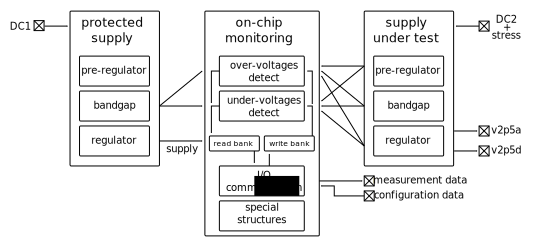
\includegraphics{src/3/figures/architecture_testchip.pdf}
  \caption{Global architecture of the test vehicle}
  \label{architecture_testchip}
\end{figure}

% What is in the monitoring system
The monitoring system is comprised of several functions.
The overvoltage and undervoltage detectors monitor several key voltages inside the supply under test.
There are in total 35 detectors in the testchip.
The communication function performs a parallel to serial conversion, in order to read and write a large amount of bits using just a few pins.
Special structures for specific monitoring functions is also implemented.
Details about the monitored and monitoring functions are given in the next sub-sections.

%TODO: Show da layout, explain a little

\subsection{Supply function under monitoring}

% Main task
The main function of the supply block is mostly to down-convert a battery voltage to a 2.5V regulated supply.
Several blocks are involved for processing the battery supply.
The overall architecture is given in fig. \ref{fig:monitored_function}).

% First block
First, a pre-regulator clamps the battery voltage that can reach 40V down to a 9V.
This is done to protect more sensitive circuits connected downstream.
This output has low current capability and is used for low-power functions.
A second output provides a 12V clamped output with a large current capability.

% Second block
A bandgap reference is connected downstream.
It is powered by the 9V supply.
Once properly started after a certain delay, the bandgap generates a 1.23 V voltage reference.
This reference is stable accross a wide range of temperature, process variation and process mismatchs.
The bandgap also outputs a 10uA current reference, and a flag \textit{bgok} to signal it is ready for operation.

\begin{figure}[!htbp]
  \centering
  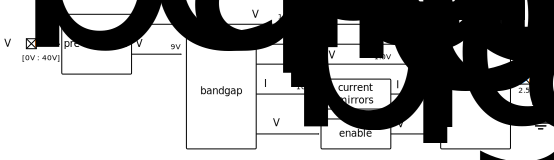
\includegraphics[width=0.9\textwidth]{src/3/figures/monitored_function.pdf}
  \caption{Architecture of the supply under test}
  \label{fig:monitored_function}
\end{figure}

% Third major block
Finally, the \gls{ldo} regulator generates a stable 2.5V supply voltage, able to deliver and sustain up to 20mA.
In the original product, this output is used further in the system to power digital gates.

% Detail nets connections
The regulator relies on multiple signals generated in the upstream blocks for operation.
The most critical nets are the 1.0V reference from the bandgap, and the ramp-up signal.
Circuit analysis show that both nets can directly affect the output voltage.
A variation on the reference voltage is immediately copied on the output.
The ramp-up signal controls the soft-start of the regulator, that can directly change the output value.
Other nets provide bias to the regulator, and their impact on the output is more limited.

% Talk about external devices
The regulator is connected externally to a 100nF decoupling capacitor to absorb peak currents and achieve stability.

% What are the minor blocks doing
The \textit{current mirrors} provide copied current values from the bandgap, while offering much larger output impedance.
The \textit{enable} block mostly checks and waits for the bandgap to be properly started.
It then triggers a startup ramp-up sequence on the regulator.

\subsection{Voltage monitoring}

% What are the OV/UV detectors made of
Overvoltage and undervoltage detectors are implemented as latched comparators.
A flag is raised if a monitored net crosses a threshold, and stored using a latch, until it can be read.
The architecture of a single detector is given Fig. \ref{fig:architecture-ov}.
The same architecture is used for the overvoltage and the undervoltage.
Monitored and reference inputs are just inversed on the undervoltage detector.

\begin{figure}[!htbp]
  \centering
  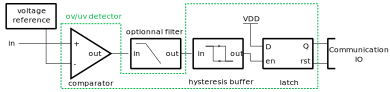
\includegraphics[width=0.9\textwidth]{src/3/figures/architecture_OV.pdf}
  \caption{Architecture of the overvoltage detector}
  \label{fig:architecture-ov}
\end{figure}

% Detail architecture
The first block in this detector is the comparator.
It is designed with a two-stage operational amplifier with an output buffer (see Fig. \ref{fig:comparator-design}).
This topology is well suited for high-gain, open-loop comparators.
This comparator provides a very high output impedance, to ensure the monitored net is not disturbed.
A high-gain is useful for limiting the comparator's offset.
The performance of the comparator is given in table \ref{tab:comparator-performance}.
The critical factors are the high to low delay, to detect very fast transients, and the offset, to ensure detection accuracy is good.

\begin{figure}[!htbp]
  \centering
  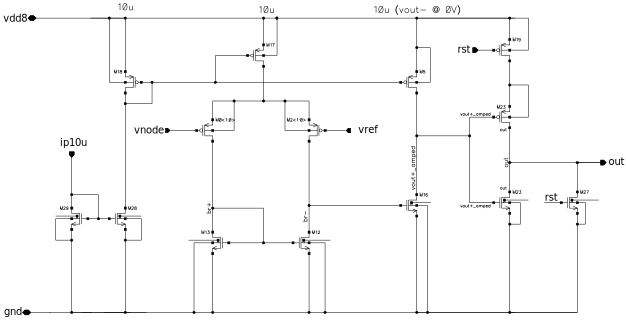
\includegraphics[width=0.9\textwidth]{src/3/figures/comparator_design_clean.pdf}
  \caption{Comparator design}
  \label{fig:comparator-design}
\end{figure}

\begin{table}[!htbp]
\centering
\begin{tabular}{@{}lllll@{}}
\toprule
property           & specification & value (typical) \\
\midrule
offset             & +/- 10mV      & 2.65 mV \\
V(IH)              & +/- 10mV      & 1.15 mV \\
V(IL)              & +/- 10 mV     & 4.16 mV \\
delay low2high     & 50 ns         & 41 ns   \\
delay high2low     & 50 ns         & 12.8 ns \\
consumption (dc)   & 60 uA         & 33 uA \\
consumption (peak) & 350 uA        & 264 uA \\
\bottomrule
\end{tabular}
\caption{Comparator performance (typical)}
\label{tab:comparator-performance}
\end{table}


% What is the purpose of filter
On the output of the comparator, an optional RC filter can be connected.
This filter can deglitch very short overvoltages, to only let large overvoltages pass through the detector.
The stratety behind this filter is to use multiple detectors monitoring the same net, each one with a different filter.
In function of which detectors triggered, an estimation of the overvoltage length can be made.

% Hysteresis buffer
After the filter, an hysteresis buffer increases the deglitching action of the filter.
If the comparator's output remains high for a short period of time, the output of the filter will rise slowly.
If a standard buffer was used in place of the hysteresis buffer, it would latch at about half the supply voltage.
With the hysteresis, the buffer switches at a voltage much closer from the supply.
With the same RC filter, this results in a much longer deglitching time.
This was done because RC-filters require large resistors and large capacitors for integration on silicon, and occupy a considerable area on the chip.
By increasing the deglitching time, smaller RC-filters could be used.

% Latch
Finally, the latch stores the overvoltage flag.
By default, the latch is reset at `0`.
Its copy input `D` is connected to the supply.
If the hysteresis buffer triggers high, the enable pin will trigger a copy in the latch.
The output `Q` will copy the value from the input `D`, storing a logical high in the latch.

% Origin of reference voltages
%TODO: DETAIL
The reference voltages for these comparators come from the protected supply.
Or DACs ?

%TODO: Designs of other blocks ?

\subsection{Communication system}

% Why a comm IO
The testchip requires many pins for basic functionnality, such as supplies, grounds, substrate connections, regulation functions.
The manufacturing process for test vehicles enforces an LQFP-48 package.
With the given requirements, this does not leave much pins available for directly outputting monitoring data.
A communication bus was designed to reduce the pin count.

% What does the comm IO
Two read-only and two write-only communication buses are implemented on the testchip.
Read-only buses are connected to overvoltage and undervoltage detectors, for reading them.
Write-only buses are connected to configuration registers for some monitoring functions.
For instance, the variable voltage references for the detectors can be set using this bus.

% Why two buses each
A pair of read/write bus serves to validate some monitoring blocks.
The second pair is connected to the actual monitoring function.

% Overall architecture
Each bus is constituted of individual identical cells.
The main principle is to propagate an enable signal.
Each time a cell receives the enable signal, it will perform its duty, wait for a delay, then pass the enable to the next cell.
%TODO: Talk about scalability
%TODO: Speak about JTAG
%TODO: Explain why custom solution and not digital-synthesis

\subsubsection{Read cell}

% Explain behavior
The read cell is constituted of a tri-state buffer and a D-latch (see Fig. \ref{fig:read-cell-design}).
The output of the tri-state buffer is set in high-impedance when the \textit{x} input is LOW.
This action releases the communication bus for other read cells and is the default state.

% Explain time-response
When the \textit{en} input goes HIGH, the output of the latch switches high at the next clock cycle.
During one clock cycle, the \textit{x} sign is HIGH and the \textit{flag} is written on the reading \textit{bus}.
At the next clock cycle, the \textit{en} signal is set low (by the previous cell).
The latch copies the LOW value, and the \textit{x} signal goes LOW, effectively releasing the bus.

\begin{figure}[!htbp]
  \centering
  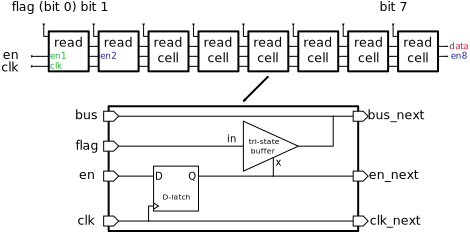
\includegraphics[width=0.5\textwidth]{src/3/figures/architecture_read_cell.pdf}
  \caption{Read-only cell design}
  \label{fig:read-cell-design}
\end{figure}

% Chaining
Multiple cells can be connected in a chain.
Increasing the total register size is simply done by adding more cells to the chain.
This is convenient for testchip developments that have limited design resources.

\subsubsection{Write cell}

% Explain behavior
The write cell is a bit more complex but operates on the same principle (Fig. \ref{fig:write-cell-design}).
Data is placed serially by the user on the \textit{bus} line, syncronously with the clock.
The enable signal is propagated from cell to cell, so that each cell can know when to sample the bus line and store the value.

\begin{figure}[!htbp]
  \centering
  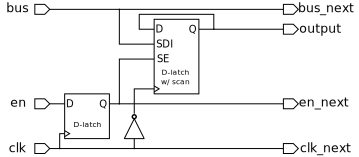
\includegraphics[width=0.5\textwidth]{src/3/figures/architecture_write_cell.pdf}
  \caption{Write-only cell design}
  \label{fig:write-cell-design}
\end{figure}

% Detail operation

% Truth table of scan D latch

\subsubsection{Register map}

%TODO
Register table

\subsection{On-chip near-field current sensors}

To be done
%TODO: Refer to PhD Alain
%TODO: Use document These/07
